\section{Methodology}
\lhead{\leftmark}
The equipment needed and procedures undertaken to carry out Electrodischarge Machining are described in the following sections. The experiment was done at ENW-04 (Machine Shop) at the JKUAT Workshops.
\subsection{Equipment}
\begin{enumerate}
\item EDM Machine (Joemars AWT 6S Wire Erosion Machine) - Figure \ref{fig:edmmachine}
\item Workpiece design as specified by the manual
\item EDM Machine controller 
\item Workpiece - 1mm mild steel sheet
\end{enumerate}
\begin{figure}[h!]
	\centering
	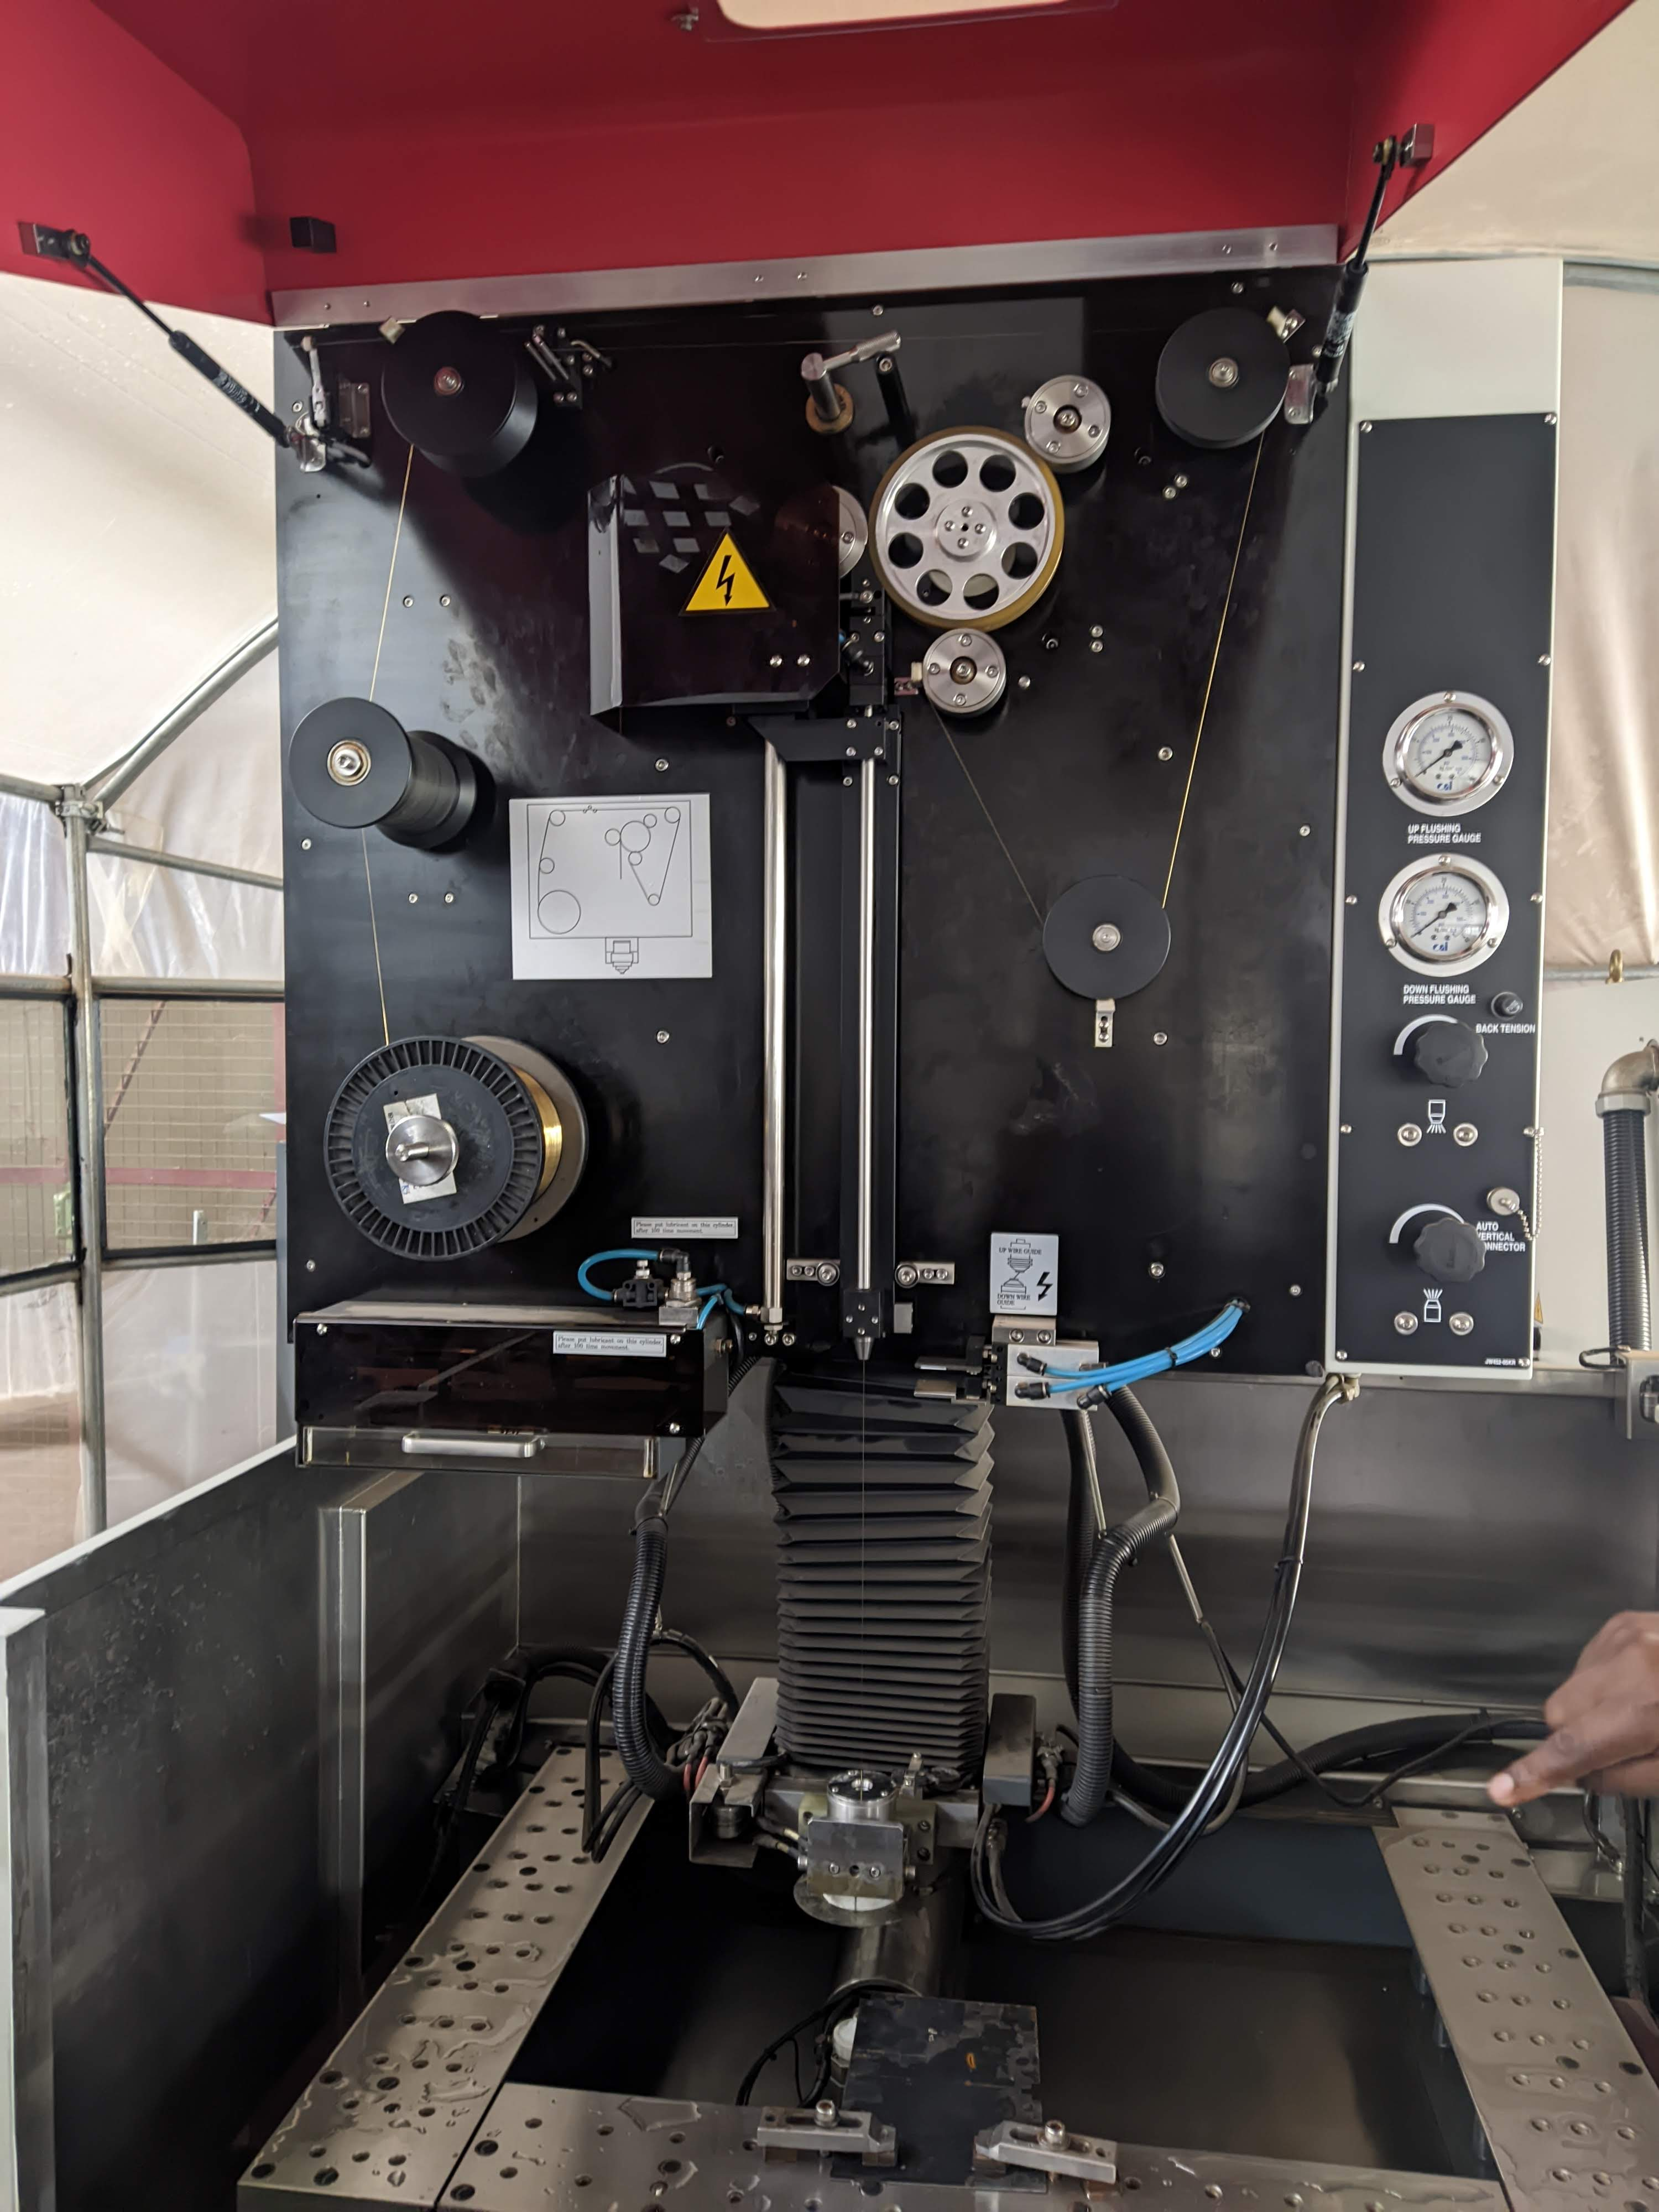
\includegraphics[width=0.7\linewidth]{Figures/edmmachine}
	\caption[EDM Machine]{Electrodischarge Machine}
	\label{fig:edmmachine}
\end{figure}
\subsection{Procedure}
Prior to beginning the machining operation, the machine is checked for any defects such as a broken wire electrode. The dielectric tank is also drained to allow access to the work table for placement and orientation of the workpiece.\\
The shape to be created was analysed and the dimensions obtained. A toolpath was created using G codes to control the EDM Machine. The codes were programmed into the EDM Machine.\\
Once the program was loaded in the machine, the wire electrode was carefully placed at a small distance from the edge of the workpiece. The pump was then turned on and the dielectric fluid, in this case water, was used to fill the dielectric tank. Once the water level reached the trigger floaters, the machine was ready to begin the machining process, thus was turned on and the machining process done. The cutting process while underway is as shown in Figure \ref{fig:cutting}\\
Once the machining process was completed, the tank was once again drained and the workpiece retrieved for examination.
\begin{figure}[h!]
	\centering
	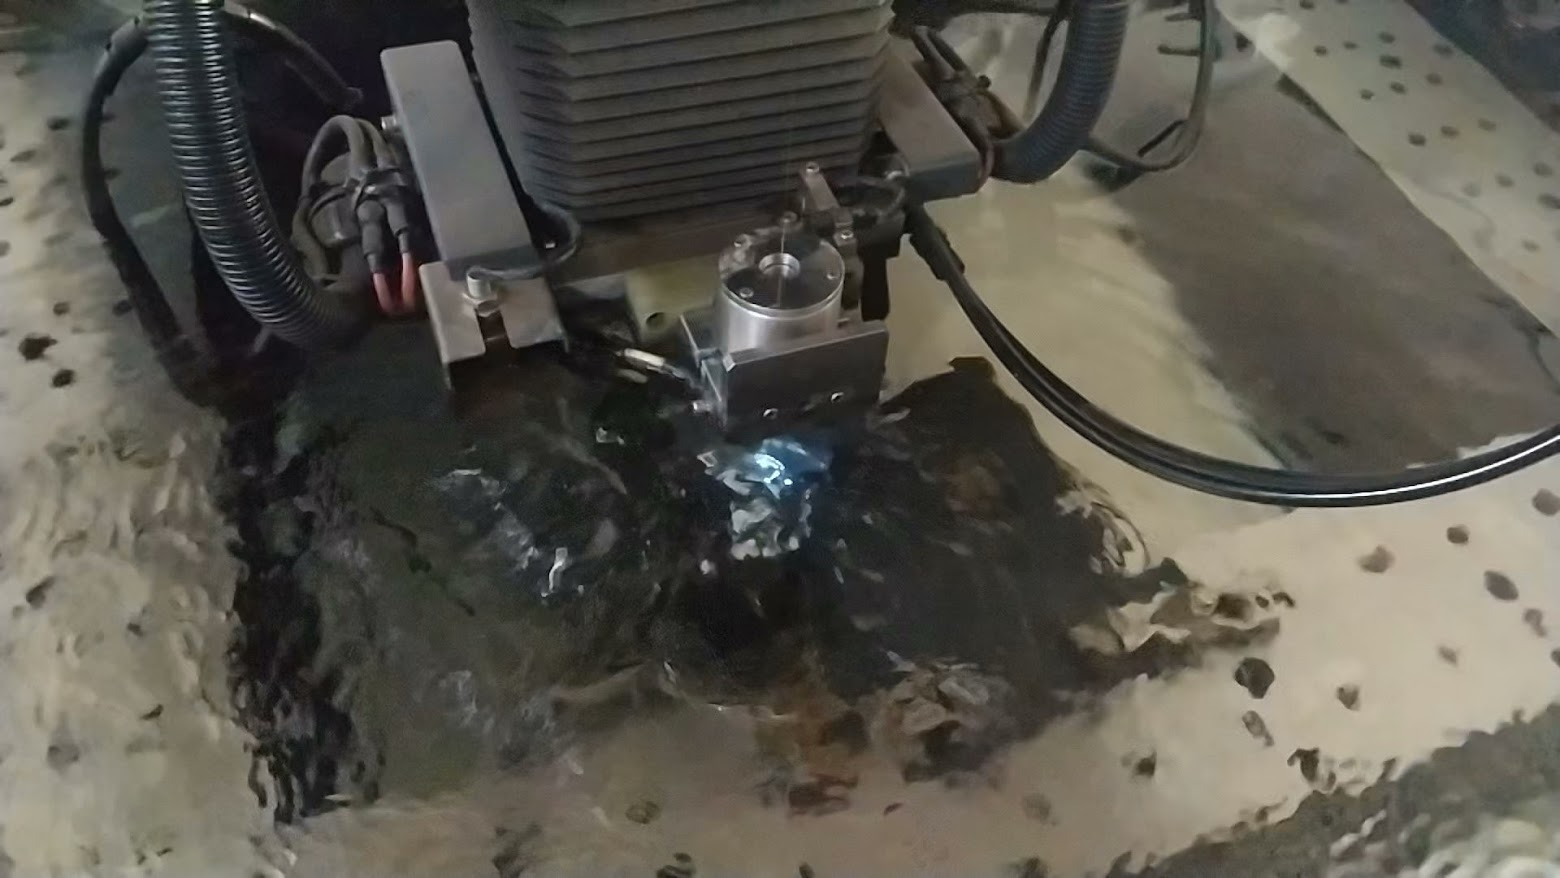
\includegraphics[width=0.7\linewidth]{Figures/edmmachining}
	\caption[EDM Machining Process]{Electrodischarge Machining Process Underway}
	\label{fig:cutting}
\end{figure}
\newpage
\subsection{EDM Machining Program}
The program used to machine the workpiece was  handwritten and then transferred to the EDM Machine Controller. The program is as follows:
\\
\begin{verbatim}
	G21
	G92 X0.0 Y0.0
	S1D1
	G01 X7.0 Y0.0
	G01 X0.0 Y-7.0
	G01 X-7.0 Y0.0
	G00 X0.0 Y0.0
	M02
\end{verbatim}